
\documentclass[
	final,      % state of work (final/draft)
	12pt,       % font size
	a4paper,
	oneside,     % twoside/oneside %PAGESTYLE
	bibliography=notnumbered,
	chapterprefix
%]{scrartcl}
]{scrreprt}

\usepackage{scrhack}
\usepackage[T1]{fontenc} 
\usepackage[utf8]{inputenc}

\usepackage[english]{babel}



%author & title:
\newcommand{\titleA}{Analysis and Implementation of Iterative}
\newcommand{\titleB}{Information Bottleneck and Agglomerative}
\newcommand{\titleSubA}{Information Bottleneck}

\newcommand{\titleSubmitted}{\today{}} 
\newcommand{\titleReviewerA}{Dipl.-Ing Clemens-Konrad Müller}
\newcommand{\titleReviewerB}{Prof. Dr.-Ing. Volker Kühn} 
\newcommand{\titleName}{Obinna Hilary Isiwekpeni \rule[-2bp]{1bp}{11bp} Albert-Einstein-Straße 22 \rule[-2bp]{1bp}{11bp} 18059 Rostock}
\newcommand{\titleMatrikel}{218204763}

%title and author are also define for package "hyperref"!!!

% load and configure packages:
% IEEE packages ---------------------------------------------------------------------

% Some very useful LaTeX packages include:
% (uncomment the ones you want to load)


% *** MISC UTILITY PACKAGES ***
%
%\usepackage{ifpdf}
% Heiko Oberdiek's ifpdf.sty is very useful if you need conditional
% compilation based on whether the output is pdf or dvi.
% usage:
% \ifpdf
%   % pdf code
% \else
%   % dvi code
% \fi
% The latest version of ifpdf.sty can be obtained from:
% http://www.ctan.org/tex-archive/macros/latex/contrib/oberdiek/
% Also, note that IEEEtran.cls V1.7 and later provides a builtin
% \ifCLASSINFOpdf conditional that works the same way.
% When switching from latex to pdflatex and vice-versa, the compiler may
% have to be run twice to clear warning/error messages.






% *** CITATION PACKAGES ***
%
\usepackage{cite}
% cite.sty was written by Donald Arseneau
% V1.6 and later of IEEEtran pre-defines the format of the cite.sty package
% \cite{} output to follow that of IEEE. Loading the cite package will
% result in citation numbers being automatically sorted and properly
% "compressed/ranged". e.g., [1], [9], [2], [7], [5], [6] without using
% cite.sty will become [1], [2], [5]--[7], [9] using cite.sty. cite.sty's
% \cite will automatically add leading space, if needed. Use cite.sty's
% noadjust option (cite.sty V3.8 and later) if you want to turn this off.
% cite.sty is already installed on most LaTeX systems. Be sure and use
% version 4.0 (2003-05-27) and later if using hyperref.sty. cite.sty does
% not currently provide for hyperlinked citations.
% The latest version can be obtained at:
% http://www.ctan.org/tex-archive/macros/latex/contrib/cite/
% The documentation is contained in the cite.sty file itself.






% *** GRAPHICS RELATED PACKAGES ***
%
\usepackage{graphicx}
%add path for PC
\graphicspath{{/Users/obinnaisiwekpeni/Desktop/Information-Bottleneck/Final_Report/files_graphics/}}
%{J:/Masterarbeit/Latex/MA_template/files_graphics/}
% *** MATH PACKAGES ***
%
\usepackage[cmex10]{amsmath}
\usepackage{amssymb}
\usepackage{mathtools}
% A popular package from the American Mathematical Society that provides
% many useful and powerful commands for dealing with mathematics. If using
% it, be sure to load this package with the cmex10 option to ensure that
% only type 1 fonts will utilized at all point sizes. Without this option,
% it is possible that some math symbols, particularly those within
% footnotes, will be rendered in bitmap form which will result in a
% document that cannot be IEEE Xplore compliant!
%
% Also, note that the amsmath package sets \interdisplaylinepenalty to 10000
% thus preventing page breaks from occurring within multiline equations. Use:
%\interdisplaylinepenalty=2500
% after loading amsmath to restore such page breaks as IEEEtran.cls normally
% does. amsmath.sty is already installed on most LaTeX systems. The latest
% version and documentation can be obtained at:
% http://www.ctan.org/tex-archive/macros/latex/required/amslatex/math/





% *** SPECIALIZED LIST PACKAGES ***
%


%%%%%%%%%%%%%%%%%%%%%%%%%%%%%%%%%%%%%%%%%%%%%%%%%%%%%%%%%%%%%%
\usepackage[german,linesnumbered,boxed,hangingcomment]{algorithm2e}
\SetKwRepeat{Tue}{Tue}{solange}% define do while loop
\SetKwComment{Comment}{$\triangleright$\ }{} %change comment style
%example:
%\Tue{Endbedingung}{
     % mache diese Sachen\;
 %   }
%%%%%%%%%%%%%%%%%%%%%%%%%%%%%%%%%%%%%%%%%%%%%%%%%%%%%%%%%%%%%%

% *** ALIGNMENT PACKAGES ***
%
%\usepackage{array}
% Frank Mittelbach's and David Carlisle's array.sty patches and improves
% the standard LaTeX2e array and tabular environments to provide better
% appearance and additional user controls. As the default LaTeX2e table
% generation code is lacking to the point of almost being broken with
% respect to the quality of the end results, all users are strongly
% advised to use an enhanced (at the very least that provided by array.sty)
% set of table tools. array.sty is already installed on most systems. The
% latest version and documentation can be obtained at:
% http://www.ctan.org/tex-archive/macros/latex/required/tools/


%\usepackage{mdwmath}
%\usepackage{mdwtab}
% Also highly recommended is Mark Wooding's extremely powerful MDW tools,
% especially mdwmath.sty and mdwtab.sty which are used to format equations
% and tables, respectively. The MDWtools set is already installed on most
% LaTeX systems. The lastest version and documentation is available at:
% http://www.ctan.org/tex-archive/macros/latex/contrib/mdwtools/


% IEEEtran contains the IEEEeqnarray family of commands that can be used to
% generate multiline equations as well as matrices, tables, etc., of high
% quality.


%\usepackage{eqparbox}
% Also of notable interest is Scott Pakin's eqparbox package for creating
% (automatically sized) equal width boxes - aka "natural width parboxes".
% Available at:
% http://www.ctan.org/tex-archive/macros/latex/contrib/eqparbox/





% *** SUBFIGURE PACKAGES ***
%\usepackage[tight,footnotesize]{subfigure}
\usepackage{subfigure} 
% subfigure.sty was written by Steven Douglas Cochran. This package makes it
% easy to put subfigures in your figures. e.g., "Figure 1a and 1b". For IEEE
% work, it is a good idea to load it with the tight package option to reduce
% the amount of white space around the subfigures. subfigure.sty is already
% installed on most LaTeX systems. The latest version and documentation can
% be obtained at:
% http://www.ctan.org/tex-archive/obsolete/macros/latex/contrib/subfigure/
% subfigure.sty has been superceeded by subfig.sty.



%\usepackage[caption=false]{caption}
%\usepackage[font=footnotesize]{subfig}
% subfig.sty, also written by Steven Douglas Cochran, is the modern
% replacement for subfigure.sty. However, subfig.sty requires and
% automatically loads Axel Sommerfeldt's caption.sty which will override
% IEEEtran.cls handling of captions and this will result in nonIEEE style
% figure/table captions. To prevent this problem, be sure and preload
% caption.sty with its "caption=false" package option. This is will preserve
% IEEEtran.cls handing of captions. Version 1.3 (2005/06/28) and later
% (recommended due to many improvements over 1.2) of subfig.sty supports
% the caption=false option directly:
%\usepackage[caption=false,font=footnotesize]{subfig}
%
% The latest version and documentation can be obtained at:
% http://www.ctan.org/tex-archive/macros/latex/contrib/subfig/
% The latest version and documentation of caption.sty can be obtained at:
% http://www.ctan.org/tex-archive/macros/latex/contrib/caption/




% *** FLOAT PACKAGES ***
%
%\usepackage{fixltx2e}
% fixltx2e, the successor to the earlier fix2col.sty, was written by
% Frank Mittelbach and David Carlisle. This package corrects a few problems
% in the LaTeX2e kernel, the most notable of which is that in current
% LaTeX2e releases, the ordering of single and double column floats is not
% guaranteed to be preserved. Thus, an unpatched LaTeX2e can allow a
% single column figure to be placed prior to an earlier double column
% figure. The latest version and documentation can be found at:
% http://www.ctan.org/tex-archive/macros/latex/base/



%\usepackage{stfloats}
% stfloats.sty was written by Sigitas Tolusis. This package gives LaTeX2e
% the ability to do double column floats at the bottom of the page as well
% as the top. (e.g., "\begin{figure*}[!b]" is not normally possible in
% LaTeX2e). It also provides a command:
%\fnbelowfloat
% to enable the placement of footnotes below bottom floats (the standard
% LaTeX2e kernel puts them above bottom floats). This is an invasive package
% which rewrites many portions of the LaTeX2e float routines. It may not work
% with other packages that modify the LaTeX2e float routines. The latest
% version and documentation can be obtained at:
% http://www.ctan.org/tex-archive/macros/latex/contrib/sttools/
% Documentation is contained in the stfloats.sty comments as well as in the
% presfull.pdf file. Do not use the stfloats baselinefloat ability as IEEE
% does not allow \baselineskip to stretch. Authors submitting work to the
% IEEE should note that IEEE rarely uses double column equations and
% that authors should try to avoid such use. Do not be tempted to use the
% cuted.sty or midfloat.sty packages (also by Sigitas Tolusis) as IEEE does
% not format its papers in such ways.


%\ifCLASSOPTIONcaptionsoff
%  \usepackage[nomarkers]{endfloat}
% \let\MYoriglatexcaption\caption
% \renewcommand{\caption}[2][\relax]{\MYoriglatexcaption[#2]{#2}}
%\fi
% endfloat.sty was written by James Darrell McCauley and Jeff Goldberg.
% This package may be useful when used in conjunction with IEEEtran.cls'
% captionsoff option. Some IEEE journals/societies require that submissions
% have lists of figures/tables at the end of the paper and that
% figures/tables without any captions are placed on a page by themselves at
% the end of the document. If needed, the draftcls IEEEtran class option or
% \CLASSINPUTbaselinestretch interface can be used to increase the line
% spacing as well. Be sure and use the nomarkers option of endfloat to
% prevent endfloat from "marking" where the figures would have been placed
% in the text. The two hack lines of code above are a slight modification of
% that suggested by in the endfloat docs (section 8.3.1) to ensure that
% the full captions always appear in the list of figures/tables - even if
% the user used the short optional argument of \caption[]{}.
% IEEE papers do not typically make use of \caption[]'s optional argument,
% so this should not be an issue. A similar trick can be used to disable
% captions of packages such as subfig.sty that lack options to turn off
% the subcaptions:
% For subfig.sty:
% \let\MYorigsubfloat\subfloat
% \renewcommand{\subfloat}[2][\relax]{\MYorigsubfloat[]{#2}}
% For subfigure.sty:
% \let\MYorigsubfigure\subfigure
% \renewcommand{\subfigure}[2][\relax]{\MYorigsubfigure[]{#2}}
% However, the above trick will not work if both optional arguments of
% the \subfloat/subfig command are used. Furthermore, there needs to be a
% description of each subfigure *somewhere* and endfloat does not add
% subfigure captions to its list of figures. Thus, the best approach is to
% avoid the use of subfigure captions (many IEEE journals avoid them anyway)
% and instead reference/explain all the subfigures within the main caption.
% The latest version of endfloat.sty and its documentation can obtained at:
% http://www.ctan.org/tex-archive/macros/latex/contrib/endfloat/
%
% The IEEEtran \ifCLASSOPTIONcaptionsoff conditional can also be used
% later in the document, say, to conditionally put the References on a
% page by themselves.


% *** PDF, URL AND HYPERLINK PACKAGES ***
%
%\usepackage{url}
% url.sty was written by Donald Arseneau. It provides better support for
% handling and breaking URLs. url.sty is already installed on most LaTeX
% systems. The latest version can be obtained at:
% http://www.ctan.org/tex-archive/macros/latex/contrib/misc/
% Read the url.sty source comments for usage information. Basically,
% \url{my_url_here}.


% *** Do not adjust lengths that control margins, column widths, etc. ***
% *** Do not use packages that alter fonts (such as pslatex).         ***
% There should be no has to do such things with IEEEtran.cls V1.6 and later.
% (Unless specifically asked to do so by the journal or conference you plan
% to submit to, of course. )

%base packages

%+++++++++++++++++++++++++++++++++++++++++++++++++++++++++++++++++++++++++++++++++++++++++++++++++++++++++++++++++++++++
% correct bad hyphenation here
%\addto{\captionsenglish}{
	%\renewcommand{\refname}{Bibliography} %for article class
	%\renewcommand{\bibname}{Bibliography} %for book class
%}
%\hyphenation{min-i-mi-za-tion
%}

%+++++++++++++++++++++++++++++++++++++++++++++++++++++++++++++++++++++++++++++++++++++++++++++++++++++++++++++++++++++++
% additional math-packages
\usepackage{trfsigns}
\usepackage[thinspace,thinqspace,squaren,textstyle]{SIunits}
\usepackage{bm}
\usepackage{amssymb}
\usepackage{amsmath}

%\usepackage{mathtools}
%\mathtoolsset{showonlyrefs} % use \refeq{eqlabel} or \eqref{eqlabel} to reference equations. Then only really referenced equations get a number.

%+++++++++++++++++++++++++++++++++++++++++++++++++++++++++++++++++++++++++++++++++++++++++++++++++++++++++++++++++++++++
% include geometry-packages 
\usepackage[
  a4paper, % = 210mm x 297mm
  twoside, %PAGESTYLE
  left=22mm,
  right=22mm,
  top=33mm,
  bottom=30mm,
  bindingoffset=10mm,
  headheight=15mm
 % hoffset=5mm,          % (1)  (see latex_help\layout.png )  
 % voffset=10mm,         % (2)
 % headheight=10mm,      % (5)
 % headsep=10mm,         % (6)
 % textheight=240mm,     % (7)
 % textwidth=160mm,      % (8)
 % marginparsep=10mm,    % (9)
 % marginparwidth=12mm,  % (10)
 % footskip=10mm,        % (11)
]{geometry}

%\setlength{\baselineskip}{17pt}
\renewcommand{\baselinestretch}{1} % scales the value of \baselineskip. Its default value is 1.0
%\setlength{\parskip}{\baselineskip} % distance between paragraphs
%\setlength{\parindent}{0pt} % removes indent of paragraphs

%+++++++++++++++++++++++++++++++++++++++++++++++++++++++++++++++++++++++++++++++++++++++++++++++++++++++++++++++++++++++
 %package to define headings 
\usepackage[automark]{scrpage2}
%define headings:
\pagestyle{scrheadings}
\clearscrheadfoot

%\ohead{\pagemark}
\automark[subsection]{section}
\ofoot{\pagemark}
%\ihead{Name}

%+++++++++++++++++++++++++++++++++++++++++++++++++++++++++++++++++++++++++++++++++++++++++++++++++++++++++++++++++++++++
% table packages
\usepackage{multirow}
\usepackage{longtable}	%enable support for tables over 2 pages
\usepackage[table]{xcolor} %highlight cells in a table
\usepackage{tabularx}
\newcommand{\cellcolorA}{\cellcolor[gray]{0.9}} % Highlight Cell - command
\newcommand{\cellcolorB}{\cellcolor[gray]{0.8}} % Highlight Cell - command
\newcommand{\cellcolorC}{\cellcolor[gray]{0.7}} % Highlight Cell - command
\newcommand{\cellcolorD}{\cellcolor[gray]{0.6}} % Highlight Cell - command

%+++++++++++++++++++++++++++++++++++++++++++++++++++++++++++++++++++++++++++++++++++++++++++++++++++++++++++++++++++++++
% include psfrag (replace text in figures)
\usepackage{psfrag}
\usepackage{placeins} %placeins ist ein Paket, welches verhindert, dass Floats hinter dem Befehl \FloatBarrier erscheint. 

%+++++++++++++++++++++++++++++++++++++++++++++++++++++++++++++++++++++++++++++++++++++++++++++++++++++++++++++++++++++++
% include package for new algorithm-environment
%\usepackage[Alg.,nothing]{algorithm} %25.09.2014
\usepackage{caption}%[2007/09/01]

%+++++++++++++++++++++++++++++++++++++++++++++++++++++++++++++++++++++++++++++++++++++++++++++++++++++++++++++++++++++++
%change labels
%\renewcommand{\listfigurename}{List of Figures}
%\renewcommand{\listtablename}{List of Tables}
\renewcommand{\figurename}{Fig.}
\renewcommand{\tablename}{Tab.}
\addto\captionsenglish{%
	\renewcommand{\figurename}{Fig.}
	\renewcommand{\tablename}{Tab.}
}
\newcommand{\sectionname}{Sec.}
%\newcommand{\equationname}{Eq.}

\newcommand{\etal}[0]{\textit{et al.}}
\newcommand{\refFig}[1]{Fig.~\ref{#1}}
\newcommand{\refAlg}[1]{Alg.~\ref{#1}}
\newcommand{\refPag}[1]{p.~\pageref{#1}}
\newcommand{\refApp}[1]{App., part~\ref{app:#1}}
\newcommand{\refTab}[1]{Tab.~\ref{#1}}
\newcommand{\refSec}[1]{Sec.~\ref{#1}}
\newcommand{\refCha}[1]{Ch.~\ref{cha:#1}}
\newcommand{\refEq}[1]{\eqref{#1}}

\newcommand{\labFig}[1]{\label{fig:#1}}
\newcommand{\labAlg}[1]{\label{alg:#1}}
\newcommand{\labApp}[1]{\label{app:#1}}
\newcommand{\labTab}[1]{\label{tab:#1}}
\newcommand{\labSec}[1]{\label{sec:#1}}
\newcommand{\labCha}[1]{\label{cha:#1}}
\newcommand{\labEq}[1]{\label{eq:#1}}

\numberwithin{equation}{chapter} %add section number to equations (e.g. "(1.4)" instead of "(4)")
\numberwithin{figure}{chapter}
\numberwithin{table}{chapter}
%\numberwithin{algorithm}{chapter}%25.09

%Redefine \dotfill (larger space between dots)
\makeatletter
\renewcommand*\dotfill{\leavevmode%
	\leaders\hbox{$\m@th
		\mkern \@dotsep mu\hbox{.}\mkern \@dotsep
		mu$}\hfill\kern\z@}
\makeatother
		
%+++++++++++++++++++++++++++++++++++++++++++++++++++++++++++++++++++++++++++++++++++++++++++++++++++++++++++++++++++++++
% Widows and orphans in LaTeX
% When writing in LaTeX, you sometimes experience that words or short lines of text at the beginning or end of a paragraph are printed at the bottom or top of a page. 
% This makes them separated from the rest of the text in the paragraph. Such words or lines are called widows and orphans.
% Orphans are the first words/lines of a paragraph at the end of a page and widows are the last words/lines that appear at the page top.
% Here, is a way to change the way LaTeX deal with these phenomena.
%
% The LaTeX algorithm takes these artifacts into account, but not always in a preferable way. 
% It makes use of \widowpenalty and \clubpenalty. By default, these parameters are set to a value of 150.
% Increasing these numbers, to for instance 500, makes them more important for LaTeX:
\clubpenalty=150000 
\widowpenalty=150000

%+++++++++++++++++++++++++++++++++++++++++++++++++++++++++++++++++++++++++++++++++++++++++++++++++++++++++++++++++++++++
% bibliography style


%\bibliographystyle{IEEEtran}
\bibliographystyle{alpha}

% remove default caption
%\renewcommand{\bibname}{}
%\renewcommand{\refname}{}

%+++++++++++++++++++++++++++++++++++++++++++++++++++++++++++++++++++++++++++++++++++++++++++++++++++++++++++++++++++++++
%hyperlink support 
\usepackage[
      pdfauthor={Autorenname}, 
      pdftitle={Titel der Arbeit}, 
      colorlinks=true, 
      urlcolor=black, 
      linkcolor=black,
      citecolor=black,
      pdfpagelayout=TwoPageRight,	%TwoPageRight/SinglePage %PAGESTYLE
      bookmarksnumbered,			% bookmarks in the pdf-viewer will be numbered
      bookmarksopen,				% bookmarks will be open when pdf-viewer is started
      plainpages=false,				% prevents "destination with the same identifier"-Warning
      linktocpage=true,
      %breaklinks=true
]{hyperref}

%\usepackage{breakurl}  % When you do not compile with pdflatex (e.g. because you want to use \usepackage{psfrag}), urls with hyperref are not line wrapped. This package wraps them again and remains working lins! Great particularly for bibliographies with links.

%+++++++++++++++++++++++++++++++++++++++++++++++++++++++++++++++++++++++++++++++++++++++++++++++++++++++++++++++++++++++
\usepackage{acronym}
% TexWorks hat genau hier auf einmal rumgemeckert
%\newcommand{\bflabel}[1]{\normalfont{\normalsize{#1}}\hfill} %set font of abbreviations to normal font

%% glossaries (abbreviations and symbols)
%\usepackage[
%	nonumberlist,		%do not show page numbers
%	acronym,			%list of abbreviations
%	toc,				%add labes in table of content
%	section,			%move labes in toc to same level as sections
%	hyperfirst=false	%suppress the first use link for all terms
%]{glossaries}
%
%\newglossary[slg]{symbols}{syi}{syg}{Symbols}
%\renewcommand*{\glspostdescription}{} %remove dot at the end of each description
%\makeglossaries % create glossary-files

%+++++++++++++++++++++++++++++++++++++++++++++++++++++++++++++++++++++++++++++++++++++++++++++++++++++++++++++++++++++++++
%andere Pakete
%\usepackage{amsfonts}  
%Tikz matlab figures
\usepackage{pdfpages} 
\usepackage{tikz,pgfplots}
\usetikzlibrary{calc}

%\pgfplotsset{compat=newest}
%\usepgfplotslibrary{external} 
%\tikzexternalize[prefix=TikzPictures/]
%

\usepackage{color}
\definecolor{uniblue}{rgb}{0,0.29,0.6} % könnte Probleme machen, wenn noch xcolor eingebunden ist!!!!

\usepackage{forest}
%\usetikzlibrary{positioning}
%\usetikzlibrary{trees,arrows,positioning}
\usetikzlibrary{arrows,chains,matrix,positioning,scopes}

%\tikzset{level 1/.style={level distance=3cm, sibling distance=2.5cm}}
%\tikzset{level 2/.style={level distance=4cm, sibling distance=2cm}}

%\tikzset{bag/.style={circle}}

\usepackage{rotating} 
\usepackage{longtable} 

\makeatletter
\tikzset{join/.code=\tikzset{after node path={%
\ifx\tikzchainprevious\pgfutil@empty\else(\tikzchainprevious)%
edge[every join]#1(\tikzchaincurrent)\fi}}}
\makeatother
%
\tikzset{>=stealth',every on chain/.append style={join},
         every join/.style={->}}
\tikzstyle{labeled}=[execute at begin node=$\scriptstyle,
   execute at end node=$]
%
%noch mehr andere Pakete

%Für große griechische Buchstaben wie ein großes Lambda 8.02.2016
\usepackage{ upgreek }
%für doppelt angestrichene Buchstaben für reelle, komplexe Zahlen, Erwartungswert
\usepackage{dsfont}

% load macros:
%%%%%%%%%%%%%%%%%%%%%%%%%%%%%%%%%%%%%%%%%%%%%%%%%%%%%%%%%%%%%%
%
% Used Symbols (for use in math-environment)
%
%%%%%%%%%%%%%%%%%%%%%%%%%%%%%%%%%%%%%%%%%%%%%%%%%%%%%%%%%%%%%%



%%%%%%%%%%%%%%%%%%%%%%%%%%%%%%%%%%%%%%%%%%%%%%%%%%%%%%%%%%%%%%
%
% Environments
%
%%%%%%%%%%%%%%%%%%%%%%%%%%%%%%%%%%%%%%%%%%%%%%%%%%%%%%%%%%%%%%

\newenvironment{eqnarraylong}
{
	\begin{figure*}[t]
	\begin{eqnarray}
}
{
	\end{eqnarray}
	\hrulefill
	\end{figure*}
}


%%%%%%%%%%%%%%%%%%%%%%%%%%%%%%%%%%%%%%%%%%%%%%%%%%%%%%%%%%%%%%
%
% Complex Numbers
%
%%%%%%%%%%%%%%%%%%%%%%%%%%%%%%%%%%%%%%%%%%%%%%%%%%%%%%%%%%%%%%
\newcommand{\conj}[1]{{#1}^{\ast}}
\newcommand{\real}[1]{{\Re} \left\{{#1}\right\}}
\newcommand{\imag}[1]{{\Im} \left\{{#1}\right\}}


%%%%%%%%%%%%%%%%%%%%%%%%%%%%%%%%%%%%%%%%%%%%%%%%%%%%%%%%%%%%%%
%
% Code Listing
%
%%%%%%%%%%%%%%%%%%%%%%%%%%%%%%%%%%%%%%%%%%%%%%%%%%%%%%%%%%%%%%

%\makeatletter
  %\newenvironment{Algorithm}[1]{%
    %\begin{center}
    %\captionsetup{style=ruled,type=algorithm,skip=0pt}
    %\fst@algorithm\@fs@pre
    %\caption{#1}
    %\@fs@mid\vspace{2pt}
  	%\sffamily
  %}{%
    %\vspace{2pt}\@fs@post
    %\end{center}
  %}
%\makeatother


%%%%%%%%%%%%%%%%%%%%%%%%%%%%%%%%%%%%%%%%%%%%%%%%%%%%%%%%%%%%%%
%
% Additional Colors
%
%%%%%%%%%%%%%%%%%%%%%%%%%%%%%%%%%%%%%%%%%%%%%%%%%%%%%%%%%%%%%%

\definecolor{darkcyan}{rgb}{0.004,0.2902,0.6}
\definecolor{green}{rgb}{0,0.5,0}
\definecolor{orange}{rgb}{0.91,0.48,0.08}
\definecolor{lila}{rgb}{0.75,0,0.75}
\definecolor{lightblue}{rgb}{0,0.69,0.94}
\definecolor{silver}{rgb}{0.5,0.5,0.5}


%%%%%%%%%%%%%%%%%%%%%%%%%%%%%%%%%%%%%%%%%%%%%%%%%%%%%%%%%%%%%%
%
% Title Page in Corporate Design 
% 
% call: "\maketitle"
%
% required files:
%    title_page.eps
% required packages:
%	graphicx, color
% required commands:
% 	\graphicspath{{<PATH>/}} %if graphics are in subdirectory
%	\definecolor{darkcyan}{rgb}{0.004,0.2902,0.6}
% require new commands: 
%	\newcommand{\titleSubmitted}{DATE}
%	\newcommand{\titleReviewerA}{REVIEWER1}
%	\newcommand{\titleReviewerB}{REVIEWER2}
%	\newcommand{\titleName}{NAME}
%	\newcommand{\titleMatrikel}{MATRIKEL}
%	\newcommand{\titleA}{TITLE1}
%	\newcommand{\titleB}{TITLE2}
%	\newcommand{\titleSubA}{SUBTITLE1}
%	\newcommand{\titleSubB}{SUBTITLE2}
%%%%%%%%%%%%%%%%%%%%%%%%%%%%%%%%%%%%%%%%%%%%%%%%%%%%%%%%%%%%%%
%\usepackage[T1]{fontenc}
\newcommand{\changefont}[4]{
\fontfamily{#1} \fontseries{#2} \fontshape{#3} \fontsize{#4}{#4}\selectfont}
%
%\newcommand{\corpdesigntitle}
%{ 
	%\newpage
	%\thispagestyle{empty}
%%
	%\begin{picture}(0,0)(102.5,750)
	%\psfrag{title1}[Bl][Bl][1]{\changefont{phv}{m}{n}{22}\color{darkcyan}\titleA{}}
	%\psfrag{title2}[Bl][Bl][1]{\changefont{phv}{m}{n}{22}\color{darkcyan}\titleB{}}
	%\psfrag{subtitle1}[Bl][Bl][1]{\changefont{phv}{m}{n}{14}\color{black}\titleSubA{}}
	%\psfrag{subtitle2}[Bl][Bl][1]{\changefont{phv}{m}{n}{14}\color{black}\titleSubB{}}
%%
	%\psfrag{date}[Bl][Bl][1]{\changefont{phv}{m}{n}{11}\color{black}{eingereicht am \titleSubmitted{}}}
	%\psfrag{by}[Bl][Bl][1]{\changefont{phv}{m}{n}{11}\color{black}{von}}
	%\psfrag{name}[Bl][Bl][1]{\changefont{phv}{m}{n}{11}\color{black}\titleName{}}
	%\psfrag{matrikel}[Bl][Bl][1]{\changefont{phv}{m}{n}{11}\color{black}{Matriculation No.: \titleMatrikel}}
%%
	%\psfrag{reviewer}[Bl][Bl][1]{\changefont{phv}{b}{n}{11}\color{black}{Reviewer:}}
	%\psfrag{reviewer2}[Bl][Bl][1]{\changefont{phv}{b}{n}{11}\color{black}{Second Reviewer:}}
	%\psfrag{name1}[Bl][Bl][1]{\changefont{phv}{m}{n}{11}\color{black}\titleReviewerA{}}
	%\psfrag{name2}[Bl][Bl][1]{\changefont{phv}{m}{n}{11}\color{black}\titleReviewerB{}}
	%\psfrag{university}[Bl][Bl][1]{\changefont{phv}{m}{n}{11}\color{black}{Universität Rostock}}
	%\psfrag{street1}[Bl][Bl][1]{\changefont{phv}{m}{n}{11}\color{black}{Richard-Wagner-Straße 31}}
	%\psfrag{street2}[Bl][Bl][1]{\changefont{phv}{m}{n}{11}\color{black}{Richard-Wagner-Straße 31}}
	%\psfrag{plz1}[Bl][Bl][1]{\changefont{phv}{m}{n}{11}\color{black}{18119 Rostock-Warnemünde}}
	%\psfrag{plz2}[Bl][Bl][1]{\changefont{phv}{m}{n}{11}\color{black}{18119 Rostock-Warnemünde}}
%%
	%\psfrag{Project}[Bl][Bl][1]{\changefont{phv}{b}{n}{12}\color{white}Master-Thesis}
	%\psfrag{Faculty}[Bl][Bl][1]{\changefont{phv}{b}{n}{12}\color{white}{Faculty of Computer Science and Electrical Engineering}}
%%
	%\includegraphics{title_page}
	%\end{picture}
	%\clearpage
%}

\newcommand{\corpdesigntitle}
{
        \newpage
        \thispagestyle{empty}

\begin{picture}(0,0)(51.25,750)
\begin{tikzpicture}

%\draw ($(0,0)$) rectangle ($(\paperwidth,\paperheight)$);

\node (N1) at ($(20mm,0)$) {};
\node (N2) at ($(20mm,22mm)$) {};
\node (N3) at ($(N1)+(170mm,0)$) {};
\node (N4) at ($(N2)+(170mm,0)$) {};

\fill[color=uniblue] (N1) rectangle (N4);

\node (N5) at ($(N2)+(0,215mm)$) {};
\node (N6) at ($(N4)+(0,215mm)$) {};

\draw[line width=0.75pt,rounded corners=3mm,uniblue] ($(N1)$) -- ($(N5)$) -- ($(N6)$) -- ($(N3)$);

% LOGO
\node[anchor=north west,inner sep=0] (N7) at ($(20mm,\paperheight-20mm)$) {
\includegraphics[width=115mm]{files_graphics/Universitaet_Rostock_Logo}};

% Ueberschrift
\node[anchor=north west,inner sep=0] (N8) at ($(33mm,\paperheight-75mm)$) {\changefont{phv}{m}{n}{22}\color{darkcyan}\titleA{}};
\node[anchor=north west,inner sep=0] (N9) at ($(33mm,\paperheight-75mm-30pt)$) {\changefont{phv}{m}{n}{22}\color{darkcyan}\titleB{}};
\node[anchor=north west,inner sep=0] (N9) at ($(33mm,\paperheight-75mm-30pt-30pt)$) {\changefont{phv}{m}{n}{22}\color{darkcyan}\titleSubA{}};
%\node[anchor=north west,inner sep=0] (N9) at ($(33mm,\paperheight-75mm-30pt-30pt-20pt)$) {\changefont{phv}{m}{n}{14}\color{darkcyan}\titleSubB{}};

% Reviewer
\node[anchor=north west,inner sep=0] (N10) at ($(33mm,22+30mm)$) {\changefont{phv}{m}{n}{11}\color{black} 18119 Rostock-Warnem\"{u}nde};
\node[anchor=north west,inner sep=0] (N11) at ($(0.5*\paperwidth,22+30mm)$) {\changefont{phv}{m}{n}{11}\color{black} 18119 Rostock-Warnem\"{u}nde};
\node[anchor=north west,inner sep=0] (N12) at ($(33mm,22+30mm)+1*(0,16pt)$) {\changefont{phv}{m}{n}{11}\color{black} Richard-Wagner-Stra{\ss}e 31};
\node[anchor=north west,inner sep=0] (N13) at ($(0.5*\paperwidth,22+30mm)+1*(0,16pt)$) {\changefont{phv}{m}{n}{11}\color{black} Richard-Wagner-Stra{\ss}e 31};
\node[anchor=north west,inner sep=0] (N14) at ($(33mm,22+30mm)+2*(0,16pt)$) {\changefont{phv}{m}{n}{11}\color{black} Universit\"{a}t Rostock};
\node[anchor=north west,inner sep=0] (N15) at ($(0.5*\paperwidth,22+30mm)+2*(0,16pt)$) {\changefont{phv}{m}{n}{11}\color{black} Universit\"{a}t Rostock};
\node[anchor=north west,inner sep=0] (N16) at ($(33mm,22+30mm)+3*(0,16pt)$) {\changefont{phv}{m}{n}{11}\color{black} \titleReviewerA{}};
\node[anchor=north west,inner sep=0] (N17) at ($(0.5*\paperwidth,22+30mm)+3*(0,16pt)$) {\changefont{phv}{m}{n}{11}\color{black} \titleReviewerB{}};
\node[anchor=north west,inner sep=0] (N18) at ($(33mm,22+30mm)+4*(0,16pt)$) {\changefont{phv}{b}{n}{11}\color{black} Supervisor:};
\node[anchor=north west,inner sep=0] (N19) at ($(0.5*\paperwidth,22+30mm)+4*(0,16pt)$) {\changefont{phv}{b}{n}{11}\color{black} Lead Supervisor:};

% Submitted
\node[anchor=north west,inner sep=0] (N20) at ($(33mm,22+30mm)+10*(0,16pt)$) {\changefont{phv}{m}{n}{11}\color{black} Matriculation Number  \titleMatrikel};
\node[anchor=north west,inner sep=0] (N21) at ($(33mm,22+30mm)+11*(0,16pt)$) {\changefont{phv}{m}{n}{11}\color{black} \titleName{}};
\node[anchor=north west,inner sep=0] (N22) at ($(33mm,22+30mm)+12*(0,16pt)$) {\changefont{phv}{m}{n}{11}\color{black} by};
\node[anchor=north west,inner sep=0] (N23) at ($(33mm,22+30mm)+13*(0,16pt)$) {\changefont{phv}{m}{n}{11}\color{black} Submitted on \titleSubmitted{}};

\node[anchor=south west,inner sep=0] (N24) at ($(33mm,15mm)$) 	{\changefont{phv}{m}{n}{11}\color{white} MASTERARBEIT};
\node[anchor=south west,inner sep=0] (N24) at ($(33mm,15mm)-1*(0,16pt)$) 	{\changefont{phv}{m}{n}{11}\color{white} FAKULTÄT FÜR INFORMATIK UND ELEKTROTECHNIK};

\end{tikzpicture}
\end{picture}
\clearpage
}
%%%%%%%%%%%%%%%%%%%%%%%%%%%%%%%%%%%%%%%%%%%%%%%%%%%%%%%%%%%%%%
%
% PSfrag macros
%%%%%%%%%%%%%%%%%%%%%%%%%%%%%%%%%%%%%%%%%%%%%%%%%%%%%%%%%%%%%%

%++++++++++++++++++++++++++++++++++++++++++++++++++++++++++++++++++++++++++++++++++++++++++++++++++++++++++++++
%eigene:
%Fettes A
 \def\bA{\ensuremath{\bm{A}}}
%\def\bAv{\ensuremath{\bm{A}_{\mathrm{c}}}}
%\def\bAh{\ensuremath{\bm{A}_{\mathrm{r}}}}
\def\bAh{\ensuremath{{\bm{A}^{-}}}}
\def\bAv{\ensuremath{{\bm{A}^{|}}}}
 \def\MSE{\ensuremath{\operatorname{MSE}}}
%\def\MSE{\ensuremath{\operatorname{\sigma}}}
 \def\NMSE{\ensuremath{\operatorname{NMSE}}}
%\def\NMSE{\ensuremath{\operatorname{\sigma_{\mathrm{N}}}}}
 \def\NMSEl{\ensuremath{\operatorname{NMSE_l}}}
 \newcommand{\argmin}[1]{\underset{#1}{\operatorname{argmin}}}
 \newcommand{\dznt}{\ensuremath{\Delta \bm{z}_{\mathrm{nt}}}}
 \newcommand{\dzntz}{\ensuremath{\Delta \bm{z}_{\mathrm{nt}}}}
 \newcommand{\minimize}[3]{\argmin{#1} \ &#2,  \\ \text{s.t.} \qquad &#3 \notag}
\newcommand{\minimizeB}[4]{\argmin{#1} \ &#2,  \\ \text{s.t.} \qquad &#3, \notag \\ &#4 \notag}
\newcommand{\diag}[1]{\ensuremath{\operatorname{diag}\left(#1\right)}}
\newcommand{\F}{\ensuremath{F}}
\newcommand{\Nv}{\ensuremath{{N^{|}}}}%N vertical
\newcommand{\Nh}{\ensuremath{{N^{-}}}} %N horizontal
\newcommand{\Kv}{\ensuremath{{K^{|}}}}%N vertical
\newcommand{\Kh}{\ensuremath{{K^{-}}}} %N horizontal
\newcommand{\Khy}{\ensuremath{{K^{-}_{\mathrm{Y}}}}} %N horizontal
\newcommand{\Mv}{\ensuremath{{M^{|}}}}%N vertical
\newcommand{\Mh}{\ensuremath{{M^{-}}}} %N horizontal

\newcommand{\myalgorithmiccomment}[1]{\textcolor{blue}{\textit{\% #1}}}

\DeclareMathOperator*{\argminA}{arg\,min} % Jan Hlavacek
\DeclareMathOperator*{\argmaxA}{arg\,max} % Jan Hlavacek
%\SetKwFor{Loop}{Loop}{}{EndLoop}
%\SetKw{Quit}{quit}
%\SetKw{Break}{break}
%\SetKw{Initialize}{Initialize}
%\SetKw{AND}{AND}
%++++++++++++++++++++++++++++
%Tikz einstellungen
%Spaltenbreite
\def\picWidth{0.45\textwidth}
\def\surfaceWidth{0.25\textwidth}
\def\doublePic{0.4\textwidth}
\def\doublePicS{0.35\textwidth}
\def\picScale{0.5}
\def\verySmall{0.2\textwidth}

%\numberwithin{figure}{chapter}
%\numberwithin{equation}{chapter}
\hyphenation{}

\begin{document}

\selectlanguage{english}

\pagenumbering{roman}
% make the title area
%\maketitle
\corpdesigntitle{}

%%%%%%%%%%%%%%%%%%%%%%%%%%%%%%%%%%%%%%%%%%%%%

\cleardoublepage

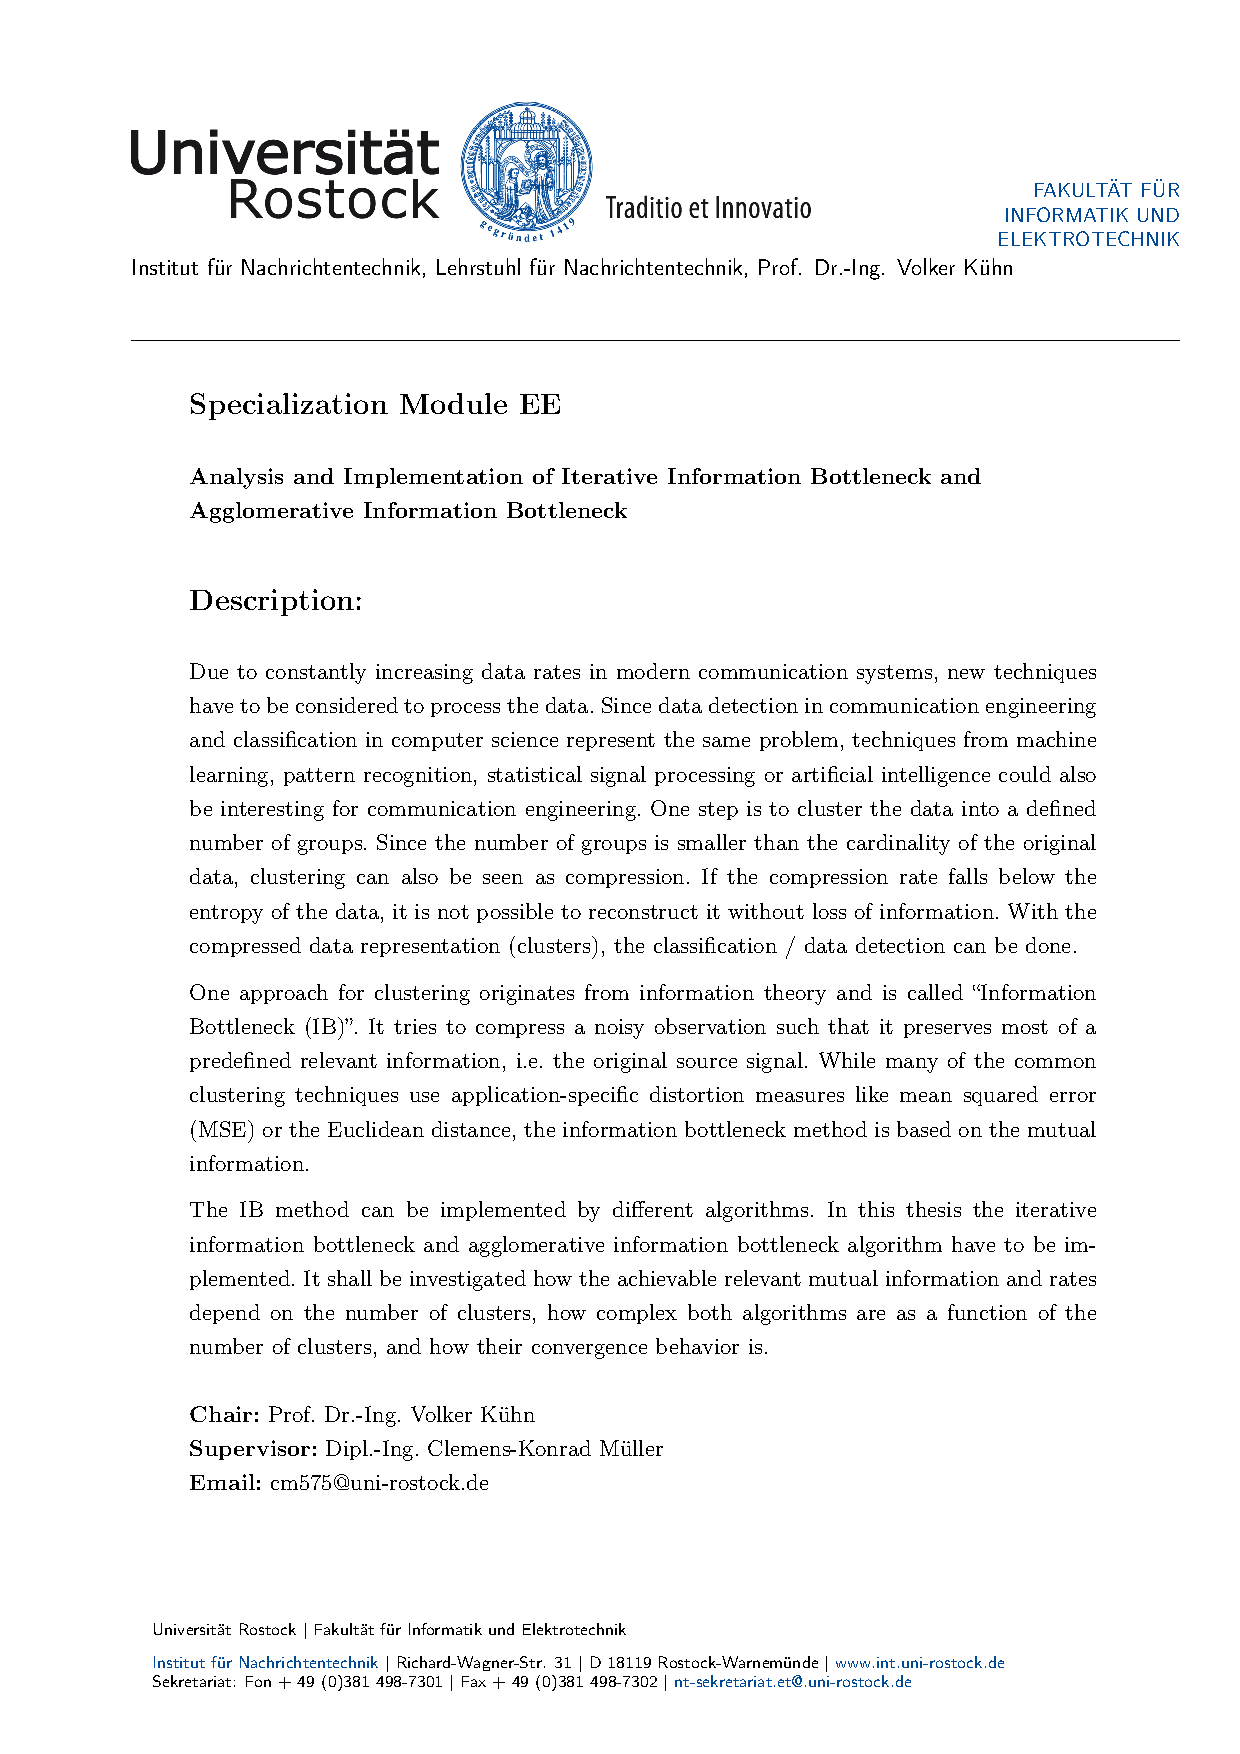
\includepdf{files_tex/IIB_aggloIB_comparison_specialization_module_topic}


%ABSTRACT

\begin{otherlanguage}{english}
\subsection*{Abstract}
\labSec{abstract_eng}
In recent times, there has been an increase in the relationship between Machine Learning and Data Communication. Clustering algorithms have some practical applications in Data Communication. There are times when data is to be transmitted from a sender to a receiver and the data is to be compressed where the compressed data should contain as much details as contained in the original information. Clustering is quite similar to compression, so it can be applied in Data Communication. One of such application is the Information Bottleneck Method. The Information Bottleneck seeks to pass data through a compact bottleneck representation. There are several algorithms used to implement the method but this report focuses on two of the algorithms which are Iterative and Agglomerative IB algorithms. The Iterative IB employs an iterative method that iterates over fixed point equations until a convergence criterion is reached. On the other hand, the Agglomerative IB employs a greedy clustering technique to find a clustering tree that goes in a bottom-up fashion.
\end{otherlanguage}



%TABLE OF CONTENT
\setcounter{tocdepth}{2}
\markboth{\contentsname}{}
\pdfbookmark[1]{\contentsname}{toc} %add table of content to pdf-bookmarks
\tableofcontents
\cleardoublepage

%GLOSSARIES

% Abbreviations
\section*{List of Abbreviations}
\addcontentsline{toc}{section}{List of Abbreviations}
\markboth{List of Abbreviations}{}
%
%\begin{acronym}[Abbreviations] 
	%\setlength{\itemsep}{-\parsep}
	%%\acro{AWGN}		{Additive White Gaussian Noise}
	%\acro{CCD} 		{Charge-coupled-device}
	%\acro{CMOS}		{Complementary metal-oxide-semiconductor}
	%\acro{CS}			{Compressed Sensing}
	%\acro{FLOP}		{Floating point operation}
	%\acro{LP}			{Linear Program}
	%\acro{MSE}		{Mean square error}
	%\acro{NMSE}		{Normed mean square error}
	%\acro{OMP}		{Orthogonal Matching Pursuit}
	%\acro{PIV}		{Particle Image Velocimetry}
	%\acro{PTV}		{Particle Tracking Velocimetry}
	%\acro{RAM}		{Random access memory}
%\end{acronym}

\begin{longtable}[l]{p{3cm} l}
IB & Information Bottleneck\\
IIB & Iterative Information Bottleneck\\
AIB & Agglomerative Information Bottleneck\\
KL & Kullback-Leibler Divergence\\
JS & Jensen-Shannon Divergence\\
SNR & Signal-to-noise ratio\\
\end{longtable}
%+++++++++++++++++++++++++++++++++++++++++++++++++++++++++++++++++++++++++++++++++++++++++++++++++++++++++++++++++++++++
% Symbols 
\section*{List of Symbols}
\addcontentsline{toc}{section}{List of Symbols}
\markboth{List of Symbols}{}
		
\renewcommand{\dotfill}{\leaders\hbox to 5pt{\hss.\hss}\hfill}



%%%%%%%%%%%%%%%%%%%%%%%%%%%%%%%%%%%%%%%%
%%%%%%%%%%%%%%%%%%%%%%%%%%%%%%%%%%%%%%%
%%%%%%%%%%%%%%%%%%%%%%%%%%%%%%%%%%%%%%%
\begin{longtable}[l]{p{3cm} l}
$H(Y)$ 									&   entropy of a variable y\\
$\textbf{A}$								&   an arbitrary matrix $A$ \\
$\beta$									&  langrange  multiplier\\
$I( X; Y)$									&  mutual information beween X and Y\\
C										&  channel capacity\\
$D_{KL}(p_1||p_2 )$							&  Kullback-Leibler Divergence between two distributions\\
$JS_{\Pi}[p_1, p_2]$							& Jensen-Shannon Divergence between two distributions\\
\end{longtable}
%%%%%%%%%%%%%%%%%%%%%%%%%%%%%%%%%%%%%%%%%%%%%%
%%%%%%%%%%%%%%%%%%%%%%%%%%%%%%%%%%%%%%%%%%%%%%%%
%%%%%%%%%%%%%%%%%%%%%%%%%%%%%%%%%%%%%%%%%%%%%%%%
%+++++++++++++++++++++++++++++++++++++++++++++++++++++++++++++++++++++++++++++++++++++++++++++++++++++++++++++++++++++++
%print glossaries

\addcontentsline{toc}{section}{List of Figures}
\listoffigures % list of figures

%\addcontentsline{toc}{section}{List of Tables}
%\listoftables  % list of tables
	
%\cleardoublepage{}
\clearpage{}

\cleardoublepage

% begin of main part +++++++++++++++++++++++++++++++++++++++++++++++++++++++++++++++++++++
\pagenumbering{arabic}

\chapter{Introduction}

Communications Engineering and Computer Science have certain things in common with respect to data transfer and communication. Data detection and classification can be seen as similar problems. In Computer science, we can use certain Machine Learning algorithms to solve such classification problems. In Communications, such problems can be solved from the Information Theory perspective by a method known as Information Bottleneck (IB). There are different algorithms that are used to implement the IB, two of which will be investigated in depth in this report. They are Iterative IB and Agglomerative IB. The basic idea of the IB method is squeezing data through a bottleneck. This is a data compression process. Given a source data which can be mapped using any of the mapping schemes (Phase Shift Keying, Amplitude Shift Keying or Quadrature Amplitude Modulation). The data is passed through an Additive White Gaussian Noise (AWGN) channel. The source data has a certain cardinality which is assigned to it. The output of the AWGN channel which is mixture of the noise and source signal has to be quantized with a quantizer which will be designed. We design the quantizer such that the output of the quantizer contains as much information as possible of the source signal. In essence, we want to maximize the mutual information between the output of the quantizer and source alphabet while keeping the mutual information between the input and output of the quantizer within a certain level. 

\section{Motivation and Goal}

The number of clusters or the cardinality affects the performance of the different IB algorithms. The goal is  to investigate how the cardinality affects the mutual information and rates of the Iterative IB and Agglomerative IB. The complexity of each algorithm with respect to the cardinality will be investigated as well their convergence behaviour.

\section{Report Outline}
\cleardoublepage

\chapter{Basic Theory}
This chapter gives an overview of the basic ideas of the building blocks of this report. A review of probability distributions is done after which basic concepts from information theory which are relevant for the implementation are introduced.

\section{Probability Density Function}
The probability density function is an important probability function that will be useful for the implementation of this pre-thesis. We shall look at the probability density function (pdf) of the distributions used in the implementation.

\subsection{Uniform Distribution}
A process is said to be uniformly distributed if all the outcomes of the process are equally likely. For example, if we have a sample space $X$ of size n, that is uniformly distributed where \(0 < n  < \infty \) then the pdf is given as

\begin{equation}
p(x) =  \begin{cases} \frac{1}{n}  & \text{for all }  x \in  \mathcal{X}  \\  0 & \text{otherwise}\end{cases}
\end{equation}

\subsection{Gaussian Distribution}
The pdf of a gaussian distribution is given as 
\begin{equation}
p(x) = \frac{1}{\sqrt{2\pi\sigma_x^2}} \e^-\frac{(x-\mu_x)^2}{2\sigma_x^2}
\end{equation}
where $\sigma_x^2$ and $\mu_x$ represent the variance and mean respectively
\section{Concepts from Information Theory}
\subsection{Entropy}
Entropy is a measure of uncertainty in a given probability distribution. Assuming we have a collection of documents and a person wants to read a single document from the collection, we would like to guess the document chosen. Without any prior knowledge, every document is equally likely. We could assume that the longer documents have a higher probability while the shorter documents have a lower probability. From the assumption, if all the documents the same number of words, then they are all equally likely. Entropy vanishes as soon as the outcome of a process is certain. The entropy of a set is maximized when all elements in the set are equally likely.
\newline
Let $Y $ be a discrete random variable distributed according to $p(y)$. The entropy of $Y$ is defined by 
\begin{equation}
H(Y) = H[p(y)] = -\sum_y p(y) \log p(y)
\end{equation}

\subsection{Mutual Information}
Given a random variable $X$ with prior probability distribution $p(x)$ and some random variable $Y$ with probability distribution $p(y)$, the mutual information is the information common to $X$ and $Y$. Reconsidering our illustration of entropy above, assuming we also consider the distinct words in the collection of documents represented by $X$ and the collection of documents as $Y$. Here, we would not only consider the prior probability distributions but also the joint distribution $p(x, y)$ which indicates the probability that a random word in the collection is equal to $x \in  \mathcal{X}$ while the particular document is  $y \in  \mathcal{Y}$.
\newline
Mutual information is the reduction of uncertainty of $X$ due to the knowledge of $Y$ and also can be defined as the information gain about $X$ due to observation of $Y$.
\begin{equation}
I(X;Y) \equiv I[p(x, y)] = \sum_x \sum_y p(x, y) \log \frac{p(x, y)}{p(x)p(y)}
\end{equation}

\subsection{Channel Capacity}
Channel capacity is the maximum rate at which data can be transmitted through a channel. It can be obtained by maximizing the mutual information $I(X;Y)$  based on the statistical properties of the source signal.  According to the channel coding theorem of Shannon, reliable communication can only be achieved up to the channel capacity.

\begin{equation}
C = \sup_{Pr\{X\}} I( X; Y)
\end{equation}

\subsection{Kullback Leibler Divergence}
It is also known as the relative entropy and it is a measure of similarity between two distributions. It is not a symmetric measure as it is not commutative. Given two probability distributions $p_1(x)$ and $p_2(x)$, the Kullback Leibler (KL) divergence between them is defined as
\begin{equation}
D_{KL}(p_1||p_2 ) = \sum_x p_1(x) \log \frac{p_1(x)}{p_2(x)}
\end{equation}
Mutual Information between two distributions can be represented in terms of their Kullback Leibler Divergence. This relationship is given as
\begin{equation}
I(X;Y) = D_{KL}[p(x, y) | p(x)p(y)]
\end{equation}
\begin{figure}
\centering
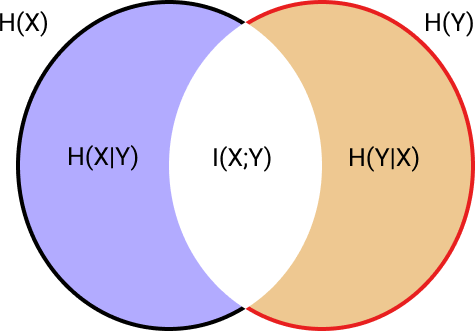
\includegraphics[scale=0.5]{Illustration_of_entropy}
\caption[Venn Diagram Illustrating Entropy and Mutual Information]{Venn Diagram Illustrating Entropy and Mutual Information: H(X) represents the entropy of X which in this case is the source signal. H(Y) represents the entropy of Y which is the sink. H(X|Y) is the entropy of X conditioned on Y. It is also called equivocation. It is the amount of information lost during transmission. H(Y|X) is known as the irrelevance i.e information not originating from the source. I(X;Y) which is the intersection of the two circles represents the mutual information }
\end{figure}
\subsection{Jensen Shannon Divergence}
This is another measure of distance between two distributions which is important for this topic. It is symmetric as opposed to KL divergence. The Jensen Shannon (JS) divergence between two probability distributions $p_1(x)$ and $p_2(x)$ is defined as
\begin{equation}
JS_{\Pi}[p_1, p_2] = \pi_1D_{KL}[p_1||\bar{p}] + \pi_2D_{KL}[p_2||\bar{p}]
\end{equation}
where \( \Pi = \{ \pi_1, \pi_2 \}, 0 < \pi_1, \pi_2 < 1, \pi_1 + \pi_2 = 1\) and  \(\bar{p} = \pi_1p_1 + \pi_2p_2\)
\subsection{Markov Chain}
Given 3 alphabets  $\mathcal{X}$, $\mathcal{Y}$ and $\mathcal{Z}$ with the relation $\mathcal{X}$ $\rightarrow$ $\mathcal{Y}$ $\rightarrow$ $\mathcal{Z}$,  since Z depends on Y, it cannot provide any "new" information about X, except the information already given by Y.

\cleardoublepage


\chapter{The Information Bottleneck Method}

\cleardoublepage

\chapter{Implementation}
This chapter shall outline the processes and steps used in implementing the Iterative IB algorithm as well as the Agglomerative IB algorithm. Python3 was used to implement both algorithms. Numpy and Matplotlib are the relevant python libraries which was used for this implementation. The Iterative IB and Agglomerative IB both have similar initial implementations just before running their individual algorithms. To keep things simple, we would start with the general implementation common to both algorithms before moving on to the individual algorithms.

\section{General Implementation}
The implementation began with importing the relevant libraries needed. The libraries imported include numpy for numerical analysis, matplotlib for plotting and data visualization, time in order to measure the time it takes for each algorithm to run. A mapper class was also imported which was used for mapping the source signal from binary to Amplitude Shift Keying (ASK) values. \\
The signal-to-noise ratio (SNR) used was 6 dB. The cardinality i.e. the number of elements of the input signal $X$ was set to 4 and real values were used for the source signal to make the investigation simple enough and not trivial by choosing a lower cardinality.  The cardinality of $Y$ which is a noisy observation of $X$ was set to be 64 which is large enough to represent $X$. \\
The cardinality of the compressed signal $Z$ which should be as large as the cardinality of X was set to 64 for the Iterative IB. For the Agglomerative IB, the cardinality of $Z$ was set to be the same cardinality of $Y$ which is 64. However the cardinality of $Z$ was varied in both algorithms in order to investigate the effect on the performance of each algorithm.\\
The input signal $X$ was modelled to be uniformly distributed that means each alphabet of the source signal is equally likely. The channel was modelled to be an Additive White Gaussian Noise (AWGN) channel. The output $Y$ of the channel is a sum of the input signal and the noise which is Gaussian distributed with zero mean and variance(power) $\sigma_{N}^2$.  The noise is Gaussian because it is assumed to be the sum of a large number of random processes which results in a Gaussian/Normal  distribution approximately if none of the individual process has a dominant effect on the variance. This is known as the \emph{Central Limit Theorem}. Hence the output of the signal is also gaussian distributed.\\
The signals were modelled to follow the Markov chain $\mathcal{X}$ $\rightarrow$ $\mathcal{Y}$ $\rightarrow$ $\mathcal{Z}$ such that $\mathcal{Z}$cannot contain more information about $\mathcal{X}$ than what is already in $\mathcal{Y}$.\\

\begin{tabularx}{1\textwidth} { 
  | >{\centering\arraybackslash}X 
  | >{\centering\arraybackslash}X 
  | >{\raggedright\arraybackslash}X | }
 \hline
 Parameter & Description & Value \\
 \hline
SNR  & Signal-to-Noise Ratio  & 6 dB \\
\hline
$N_x$  & Cardinality of X  & 4 \\
\hline
$N_y$  & Cardinality of Y  & 64 \\
\hline
$N_z$  & Cardinality of Z  & 32 for Iterative IB \newline 64 for Agglomerative IB \\
\hline
$alphabet$  & Input Alphabet & 4-ASK\\
\hline
$\sigma_{X}^2$  & Variance of source signal & 1\\
\hline
$p(x)$  & Probability of source signal & Uniform distribution\\
\hline
$p(y)$  & Probability of output signal & Gaussian distribution\\
\hline
$p(z|y)$  & Quanitizer & Initialiazed as a uniform quantizer\\
\hline
$\beta$  & Lagrangian multiplier & 0.1 to 5, 5 to 400\\
\hline
$\epsilon$  & convergence parameter & $10\e - 4$\\
\hline
\end{tabularx}
\subsection{Implementation of the Probability distributions}
The probability $p(x)$ of the source signal  $X$ was uniformly distributed while the probability $p(y)$ of the output signal $Y$ was gaussian distributed. $Y$ had to be discretized as the quantizer to be designed can only process discrete values. Then the probability of $Y$ given $X$ represented by $p(y|x)$ which in this case is the probability of the noise(AWGN) was computed. It was ensured that the sum of the conditional probability $p(y|x)$ across $Y$ yielded 1. Also the conditional probability of $X$ given $Y$  $p(x|y)$ was obtained using Bayes rule which is given as
\begin{equation}
p(x|y) = p(y|x)  \frac{p(x)}{p(y)}
\end{equation}
The joint probability  $p(x, y)$ of $X$ and $Y$ was computed by the multiplication of $p(x)$ and $p(y|x)$. The probability $p(y)$ of $Y$ was obtained by summing the joint probability $p(x, y)$  across the X. The quantizer $p(z|y)$ was initialized to be a uniform quantizer and was used to calculate $p(z)$.\\
Attention was paid to the order in which the dimensions of the matrices were assigned in order to avoid confusions. There were some situations in which the dimensions had to be expanded in order to have similar dimensions to carry out operations. For example in the computation of $p(x|z)$, $p(z|y)$ and $p(x, y)$ needed to be multiplied. Knowing the cardinality of each of the signals, the matrices were not of matching dimensions, hence the operation could not be performed leading to the use of the \emph{tile} and \emph{expanddims} functions of the numpy library. The cardinality of Z, $N_z$ was the first dimension, the cardinality of Y, $N_y$ was the second dimension while the cardinality of X, $N_x$ was the last dimension. Hence all matrices had the dimension ($N_z$, $N_y$, $N_x$). 
\section{Iterative IB}
This section details the implementation specific to the Iterative IB algorithm. The quantizer $p(z|y)$ was initialized to be a uniform quantizer with \emph{zeros} and \emph{ones} forming a step function. The Iterative IB involves  iterating through three fixed point equations and applying an update step for the next iterations.  At each step, two of the distributions are kept constant and then the algorithm that minimizes the IB function:
\begin{equation} \label{eq:1}
L[p(z | y)] = I(Y;Z) - \beta I(X;Z)
\end{equation}
At the \emph{i} + 1'th iteration, the algorithm applied an update step:
\begin{equation}
P^{(i+1)}(z|y) \leftarrow \frac{P^i(z)}{Z^{i+1}(y, \beta)}\e^-{\beta D_{KL}(p(x|y)||P^i(x|z))}
\end{equation}
where ${Z^{i+1}(y, \beta)}$ is a normalization factor. $P^i(z)$ and $P^i(x|z)$ were calculated using $P^{(i)}(z|y)$
\begin{equation}
P^i(z) = \sum_y p(y)P^{(i)}(z|y)
\end{equation}
\begin{equation}
P^i(x|z) = \frac{1}{P^i(z)}\sum_y P^{(i)}(z|y) p(x, y)
\end{equation}
The algorithm was started with a fixed $\beta$ value and smaller cardinalities of Y and Z in order to ensure it runs successfully, then gradually the cardinalities were increased and also a range of beta was used.
The  convergence parameter was set to $10\e - 4$ which was used to compare the Jensen-Shannon divergence. A \emph{while} loop was used to run the algorithm until the condition in which the Jensen-Shannon divergence was less than or equal to the convergence parameter. The Jensen-Shannon divergence measured the similarity between the previous quantizer with the current quantizer and if the value of the JS divergence between the two quantizers was less than or equal to the convergence parameter, then the present quantizer was chosen and then the Relevant Information $I(X;Z)$ and Compression Information $I(Y:Z)$ was calculated. The Relevant Information $I(X;Z)$ is upper bounded by the Mutual Information between X and Y $I(X;Y)$, while the Compression Information $I(Y:Z)$ is upper bounded by the entropy of Y $H(Y)$. 
\section{Agglomerative IB}
This section details the implementation specific to the Agglomerative IB algorithm. The algorithm uses a clustering technique to find a clustering tree in a \emph{bottom-up} fashion.  This algorithm aims at maximizing the function
\begin{equation}
L_{max} = I(X;Z) - \beta^{-1} I(Y:Z) 
\end{equation}
which is same as minimizing  equation \ref{eq:1}.
The cardinalities of $Y$ and $Z$  at the start of the algorithm were set to 64 and the aim was to carry out clustering until the desired cardinality of $Z$ which was set to 32 was achieved. To reduce the cardinality of $Z$, two values of $Z$ represented by $z_i$ and $z_j$ were iteratively merged into a single value $\bar{z}$. This was done by iterating through $p(z|y)$ which was initialized to be a uniform quantizer, hence yielding:
\begin{equation}
p(\bar{z}|y) = p(z_i|y) + p(z_j|y), \forall x \in \mathcal{X}
\end{equation}
$\bar{z}$ is simply a union of $z_i$ and $z_j$. With the Markov chain in mind, $p(\bar{z})$ was obtained by:
\begin{equation}
p(\bar{z}) = p(z_i) + p(z_j)
\end{equation}
Also, $p(x|\bar{z})$ was obtained by:
\begin{equation}
p(x|\bar{z}) = \pi_i \cdot p(x|z_i) +  \pi_ij\cdot p(x|z_j)
\end{equation}
where 
\begin{equation}
\Pi = {\pi_i, \pi_j } = {\frac{p(z_i)}{p(\bar{z}}, \frac{p(z_j)}{p(\bar{z}}},
\end{equation}
is the \emph{merger distribution}.\\
For each pair of $Z$ that was merged, the merger cost was calculated which is the difference between the values of $L_{max}$ before and after the merger. This procedure was done for all the possible mergers of $Z$ until the cardinality of 32 was reached.\\
The difference between the values of $L_{max}$ for every merger was calculated using the formula:
\begin{equation}
\Delta L_{max} (z_i, z_j) = p(\bar{z}) \cdot \bar{d}(z_i, z_j) \label{eq:2}
\end{equation}
where 
\begin{equation}
 \bar{d}(z_i, z_j) = JS_\Pi [p(x|z_i), p(x|z_j)] - \beta^(-1) JS_\Pi[p(y|z_i), p(y|z_j)]
\end{equation}
From equation \ref{eq:2}, it can be observed that the merger cost is simply a multiplication of the merged probability $p(\bar{z}) $ and the distance between them given $\bar{d}(z_i, z_j)$.
\cleardoublepage
\end{document} 
